\let\textcircled=\pgftextcircled
\chapter{Theory}
\label{chap:theory}

\initial{T}his thesis is comprised of experimental searches for dark matter and new physics. The experimental chapters Chpt.~\ref{chap:higgstoinv} and Chpt.~\ref{chap:svj} delve deeply into the analyses. Before which, the theoretical and phenomenological motivations must be understood to [back up] the need for these searches at the \acrlong{lhc}. In this chapter, a brief recap of the \acrlong{sm} will be [presented] along with its shortcomings, i.e., the lack of a dark matter candidate. Theoretical descriptions of dark matter that best fit the relic density and astrophysical observations will then be discussed. Specific interpretations in the form of \glspl{svj} and invisibly decaying Higgs bosons are [looked at] that provide the background for the respective analysis chapters.


%=========================================================


\begin{easylist}[itemize]
\ListProperties(Style*=-- , FinalMark={)}, Margin=0.5cm)
& Give an overview of the fundamental forces and particles.
& Discuss the Standard Model in detail, emphasising certain aspects as they relate to dark matter and the Higgs field (and boson).
& Briefly recap dark matter, referencing descriptions in introduction. But go into more theoretical descriptions and motivations and how they relate to potentially discovering it at the LHC (WIMP miracle).
& Discuss the theory behind the semi-visible jets analysis (main sources from Refs.~\citenum{Cohen:2015toa,Cohen:2017pzm}): strongly interacting dark sector in Hidden Valley scenario with a portal to the visible sector. Mentioning dark quarks \Pqdark, dark confinement scale \lamDark, dark hadronisation and decay, running coupling \aDark, etc.
& Explain some of the phenomenological/experimental event characteristics that overlap with both analyses, i.e., what a jet is, and maybe energy sums like \ptmiss, \HT, \htmiss, etc.
\end{easylist}


%=========================================================


\section{The standard model of particle physics}
\label{sec:standardmodel}

% Check Lancaster and other summer school notes (Postgraduate and CMS courses/ folder)


%=========================================================


\section{Limitations of the standard model}
\label{sec:sm_limitations}

% Check Lancaster and other summer school notes for other limitations, specifically referencing things that can tie into dark matter

Despite the \acrlong{sm} providing precise predictions of three of the four fundamental forces and the particles that they interact with, there are many experimental observations that it cannot currently explain. Neutrino masses, dark matter, dark energy, and gravity all escape its description.

%=========================================================


\section{Theoretical motivations for, and descriptions of, dark matter}
\label{sec:theory_dark_matter}

% Will probably be referring to things from introduction section. Try to just give overview there and describe the nitty-gritty here

The universe may have birthed dark matter via one of many possible mechanisms. The most popular is described as a ``thermal freeze-out'' process. In the hot, early universe when the thermal background allowed spontaneous pair production of particle dark matter, it was produced in abundance. During this period, they may also have frequently annihilated since the cosmos was still small. Inevitably, the universe expanded and cooled; the temperature became too low to allow significant production \cite{Baldes:2017gzw}. Matter was further separated and the dark matter annihilation rate decreased, leaving a behind the ``thermal relic'' that is observed today. These remaining particles were attracted via gravity, forming filaments throughout the universe. The potential wells they induced allowed the progenitors of galaxies to form within.

% Go into more detail about freeze-out mechanism, with some equations and plots. Could also describe freeze-in theory, 

% DON'T RENDER
\iffalse

% Taken directly from my lab book. Tidy up and improve
\begin{easylist}[itemize]
\ListProperties(Style*=-- , FinalMark={)})

& It is thought that dark matter was produced thermally in the early universe (when it was hot and therefore easier to create heavy particles). Dark matter particles could (and did) annihilate, but as the universe expanded and cooled the dark matter became more diffuse. They didn't annihilate as often and the dark matter we see today is a "thermal relic" and is what's left over. Some models suggest the parameter $x = m_{\mathrm{DM}}/T \sim 20$ at freeze out. \cite{Lisanti:2016jxe} 

& The current leading dark matter candidate is a WIMP (Weakly Interacting Massive Particle), possibly a neutral supersymmetric particle (neutralino) like a higgsino, photino, zino, etc. One of the motivations for WIMPs are that, using the current values of the dark matter density in the universe and approximations for the annihilation cross section, dark matter could self-interact at the electroweak scale to produce Standard Model particles. \cite{Kamionkowski:1997zb} As the EW scale can be readily accessed at colliders like the LHC, we could detect DM signatures via pair production then annihilation or indirect searches via solely annihilation. % Also see student seminar talk for more info on WIMP miracle

& Because WIMPs are stable (at least on the timescale of the current age of the Universe), they wouldn't decay into other particles when produced from accelerator collisions. So you would detect them (indirectly) by looking for MET and by looking for visible particles recoiling against the WIMPs.

& The mediator (force-carrying particle, like the gauge bosons) for dark matter -- between dark matter particles or the dark matter-Standard Model particle interactions -- may be a scalar (spin-0, like the Higgs boson) or pseudoscalar (reverses parity under a Lorentz transformation, like the pion) boson. [Support] for a pseudoscalar over a scalar mediator comes from the Feynman diagrams for DM annihilation into, e.g., \Pqb-quarks. With a scalar mediator, the vertex factors and the propagator term lead to cancellations in the cross section equation in the low-velocity limit.

& The mediator for dark matter may be heavier than the dark matter particle itself (like with the $W^{\pm}$ and \PZ bosons being heavier than most of the particles they mediate), maybe 2x heavier or more so than the DM particle. The mediator could decay via DM pair production, so it makes sense that it would be at least twice as heavy.

& There's no consensus on whether dark matter is fermionic or bosonic. If fermionic, it may be either a Dirac fermion (particle is distinct from its antiparticle, like the electron and positron) or Majorana fermion (particle is the same as its antiparticle, like the neutrino is \underline{suspected} to be). If it were Majorana, dark matter could annihilate with itself, making discoveries via indirect searches more likely.

& At the LHC, monojets are used most prominently to look for dark matter particles. But multijet plus \etmiss might provide better sensitivity and constraints (particularly if the mediator is pseudoscalar).

& \underline{Many} dark matter candidates include a few supersymmetric particles (the neutralino being the most widely studied), sterile neutrinos \cite{doi:10.1142/S0218301313300191}, axions, Kaluza-Klein states \cite{Han:1998sg} (which are excitations of Standard Model fields in extra dimensions), etc.

& Some good results showcasing dark matter masses and that of its mediator from different analyses and decay channels are at \cite{CMS-DP-2016-057}. Particularly figures 4 and 6, which I used in my poster for the PGR conference.

\end{easylist}


% Taken directly from my lab book. Tidy up and improve. Look through these papers to see which ones give compelling interpretations and motivation for dark matter
Papers to look at regarding SUSY and dark matter:

\begin{easylist}[itemize]
\ListProperties(Style*=, FinalMark={)})
& \cite{dmsearcheslhc2015}
& \cite{dmbenchmarkearlylhcrun2}
& \cite{CMS-PAS-EXO-12-055}
& \cite{Aitchison:2005cf}
& \cite{Ellis:2002mx}
& \cite{Murayama:2007ek}
& \cite{Peskin:2007nk}
& \cite{Goodman:2010ku}
& \cite{PhysRevLett.115.181802}
& \cite{CMS:2016pod}
& \cite{Bertone:2004pz}
\end{easylist}

\fi


%=========================================================


\section{Important observables in collider physics}
\label{sec:theory_important_observables}


%=========================================================


\subsection{Transverse momentum (\texorpdfstring{\pt}{pt})}
\label{subsec:theory_pt}

In the LHC (or any other collider), the longitudinal momentum of the initial state particles is typically unknown. However, the momentum transverse to the beam is zero before the collision, and therefore must be zero afterward after due to momentum conservation. This is why the transverse momentum of a particle or physics object (\ptvec for the vector quantity, \pt for its magnitude) is a useful variable in an analysis.

% Do I need a more formal/mathematical definition, or a diagram?


%=========================================================


\subsection{\texorpdfstring{\HT}{HT}}
\label{subsec:theory_ht}

% Will need to define what a jet is here if I don't do so before

The scalar sum of the transverse momentum of hadronic constituents in an event, i.e., the \glspl{jet}, is symbolised as \HT. It is often used in analyses focused on hadronic objects, such as natural \acrlong{susy} in which a large jet multiplicity is expected. Formally,

\begin{equation}
    \HT \equiv \sum_{\mathrm{jets}} \pt
    \label{eq:ht_definition}
\end{equation}

Typically, a lower limit on \pt is used when calculating the \HT, so jets below this threshold do not factor into the sum. This is to avoid low momentum jets attributed to pileup events (see Chpt.~\ref{subsec:pileup}), and those from the primary vertex that can often be mismeasured.


%=========================================================


\subsection{Missing transverse momentum (\texorpdfstring{\ptmiss}{ptmiss})}
\label{subsec:theory_met}

The missing transverse momentum \ptmiss is defined as the negative vector sum of the \pt of all identified particles in an event. It is a term often used interchangeably with \gls{met} (MET, \glssymbol{met}). Undetected particles from neutrinos or dark matter, or mismeasured kinematic properties of identified particles, will introduce an imbalance in the vector sum of the \pt. Hence, the \ptmiss will be non-zero. Formally,

\begin{equation}
    \ptmiss \equiv - \sum_i^{N_{\mathrm{particles}}} {\vec p}_{\mathrm{T}, \, i}
    \label{eq:met_definition}
\end{equation}

The hadronic-only counterpart to this variable, \mht, is the negative vector sum of the jet transverse momenta in an event:

\begin{equation}
    \mht \equiv - \sum_j^{N_{\mathrm{jets}}} {\vec p}_{\mathrm{T}, \, j}
    \label{eq:mht_definition}
\end{equation}

As with \HT, the \mht is often calculated with a lower limit on the jet \pt.

% A depiction of the MET (e.g., SM particles recoiling off dark matter) might be useful for the reader


%=========================================================


\section{Measuring the branching ratio of invisibly decaying Higgs bosons}
\label{sec:theory_higgs_to_inv}

% Can pull from Section 37 in my lab book, as well as all the talk I've given (Presentations and talks/ folder, my IOP one is a good starting point)
The Higgs boson has caught the attention of the high energy physics community and even the public eye like no other particle in recent memory. Its discovery in the $\PH \rightarrow \Pphoton\Pphoton$ channel in 2012 by both \acrshort{cms}~\cite{Chatrchyan:2012xdj} and \acrshort{atlas}~\cite{Aad:2012tfa} independently realised one of the [principal] goals of the LHC's construction. The particle itself is not necessarily exciting. Rather, it confirms the existence of the Higgs \emph{field} that pervades the universe and gives mass to the elementary particles via the exchange of its namesake boson~\cite{PhysRevLett.13.321,PhysRevLett.13.508,PhysRevLett.13.585}. [Its discovery], one might think, was the end of the discussion of the Higgs boson. However, it was only the beginning.

Many observations of the Higgs, such as its predominant decay mode $\PH \rightarrow \Pqb\Pqb$, were not seen until recently (\acrshort{cms}~\cite{Sirunyan:2018kst}, \acrshort{atlas}~\cite{Aaboud:2018zhk}). Constraints on its other properties have also been placed, such as its resonance width and branching ratios \BR to other final states. Fully understanding the Higgs boson is important to understanding the Higgs field and the wider \acrlong{sm}. Precision measurements in tension with \acrshort{sm} predictions can also be a window to new physics. Measuring the \higgstoinv branching ratio aims to do just that.

The only \acrshort{sm} process in which Higgs boson can decay invisibly is $\PH \rightarrow \PZ\PZ \rightarrow 4\nu$ with a branching ratio of \OrderOf{\text{0.1\,\%}}~\cite{Heinemeyer:1559921}. The leading observed experimental upper limits on this measurement are 19\,\% from CMS~\cite{Sirunyan:2018owy} and 26\,\% from \acrshort{atlas}~\cite{Aaboud:2019rtt}, far above the predicted value. If undiscovered invisible particles, perhaps dark matter, couple to the Higgs field the branching ratio will be enhanced. Experimental evidence shows the coupling strength to proportionally follow the mass of the particle, as verified in \acrshort{atlas} and \acrshort{cms}' latest measurements~\cite{Sopczak:2708121}. A considerably large enhancement may allow for this process to be observed at the \acrshort{lhc}. At the very least, a more accurate constraint on the branching ratio is able to exclude some models of dark matter, such as those described in Refs.~\citenum{Djouadi:2012zc,KAKIZAKI201544}.

There is no reason to assume dark matter does \emph{not} interact with the Higgs field, since it bestows mass to all known elementary particles (a small caveat, perhaps, being neutrinos). Higgs ``portal'' models have been theorised that connect the visible sector of the \acrlong{sm} to a dark sector where particle dark matter resides~\cite{higgs_portal_singlet_dm,Arcadi:2019lka}.

% Do I need to give a more mathematical motivation for the BR being enhanced/what kind of values the BR is expected to be from various DM models? Do I also need to give some mathematical motivation as to _why_ dark matter would couple to the Higgs? Should I add a figure/plot to break up the text? Maybe the Higgs coupling strength? Or some plot regarding Higgs coupling to dark matter?


%=========================================================


\section{Searches for semi-visible jets}
\label{sec:theory_svj}

% Can pull from Section 14 and Section 35 of my lab book, and all the talks I and other people from the team have given (Presentations and talks/ folder, also Other peoples/ subdirectory)

\begin{figure}[htbp]
\centering
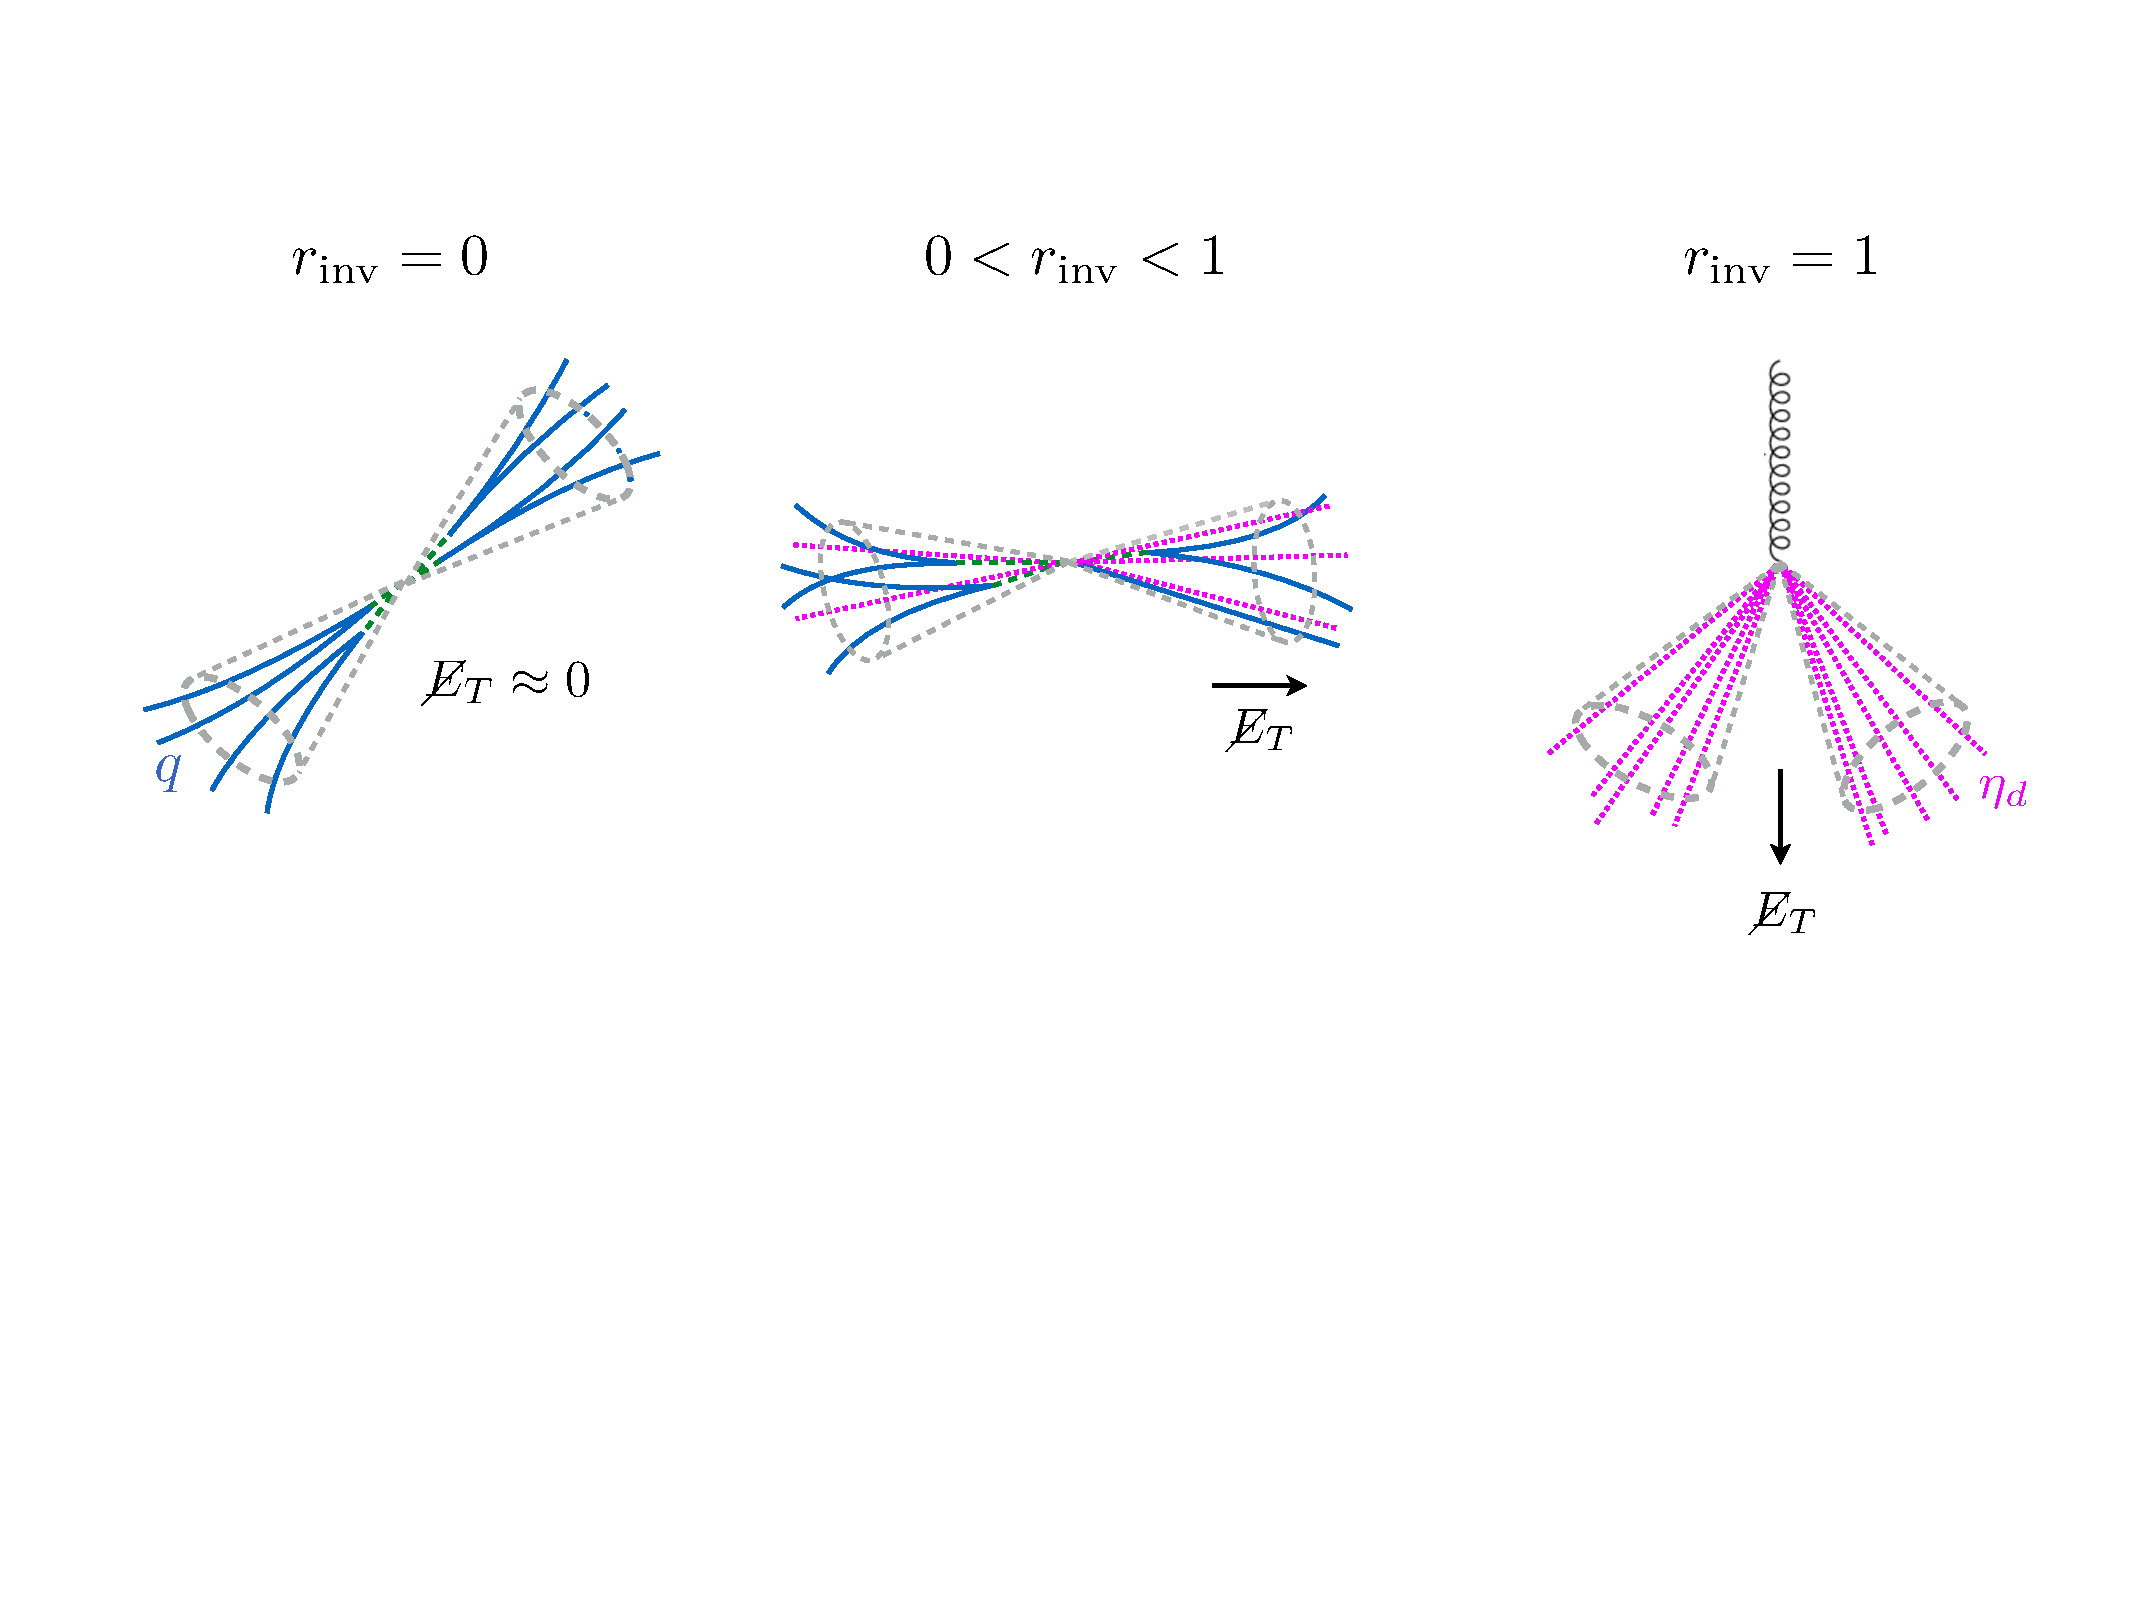
\includegraphics[width=0.85\textwidth]{figures/svj/metfigure.pdf}
\caption[The typical direction of the missing transverse energy relative to the semi-visible jets as a function of the invisible fraction \rinv]{The typical direction of the missing transverse energy \ETslash\xspace (or \ptmiss) relative to the semi-visible jets as a function of their invisible fraction \rinv \cite{Cohen:2017pzm}.}
\label{fig:theory_svj_met_dir}
\end{figure}

\begin{figure}[htbp]
    \centering
    \begin{subfigure}[c]{0.45\textwidth}
    \centering
        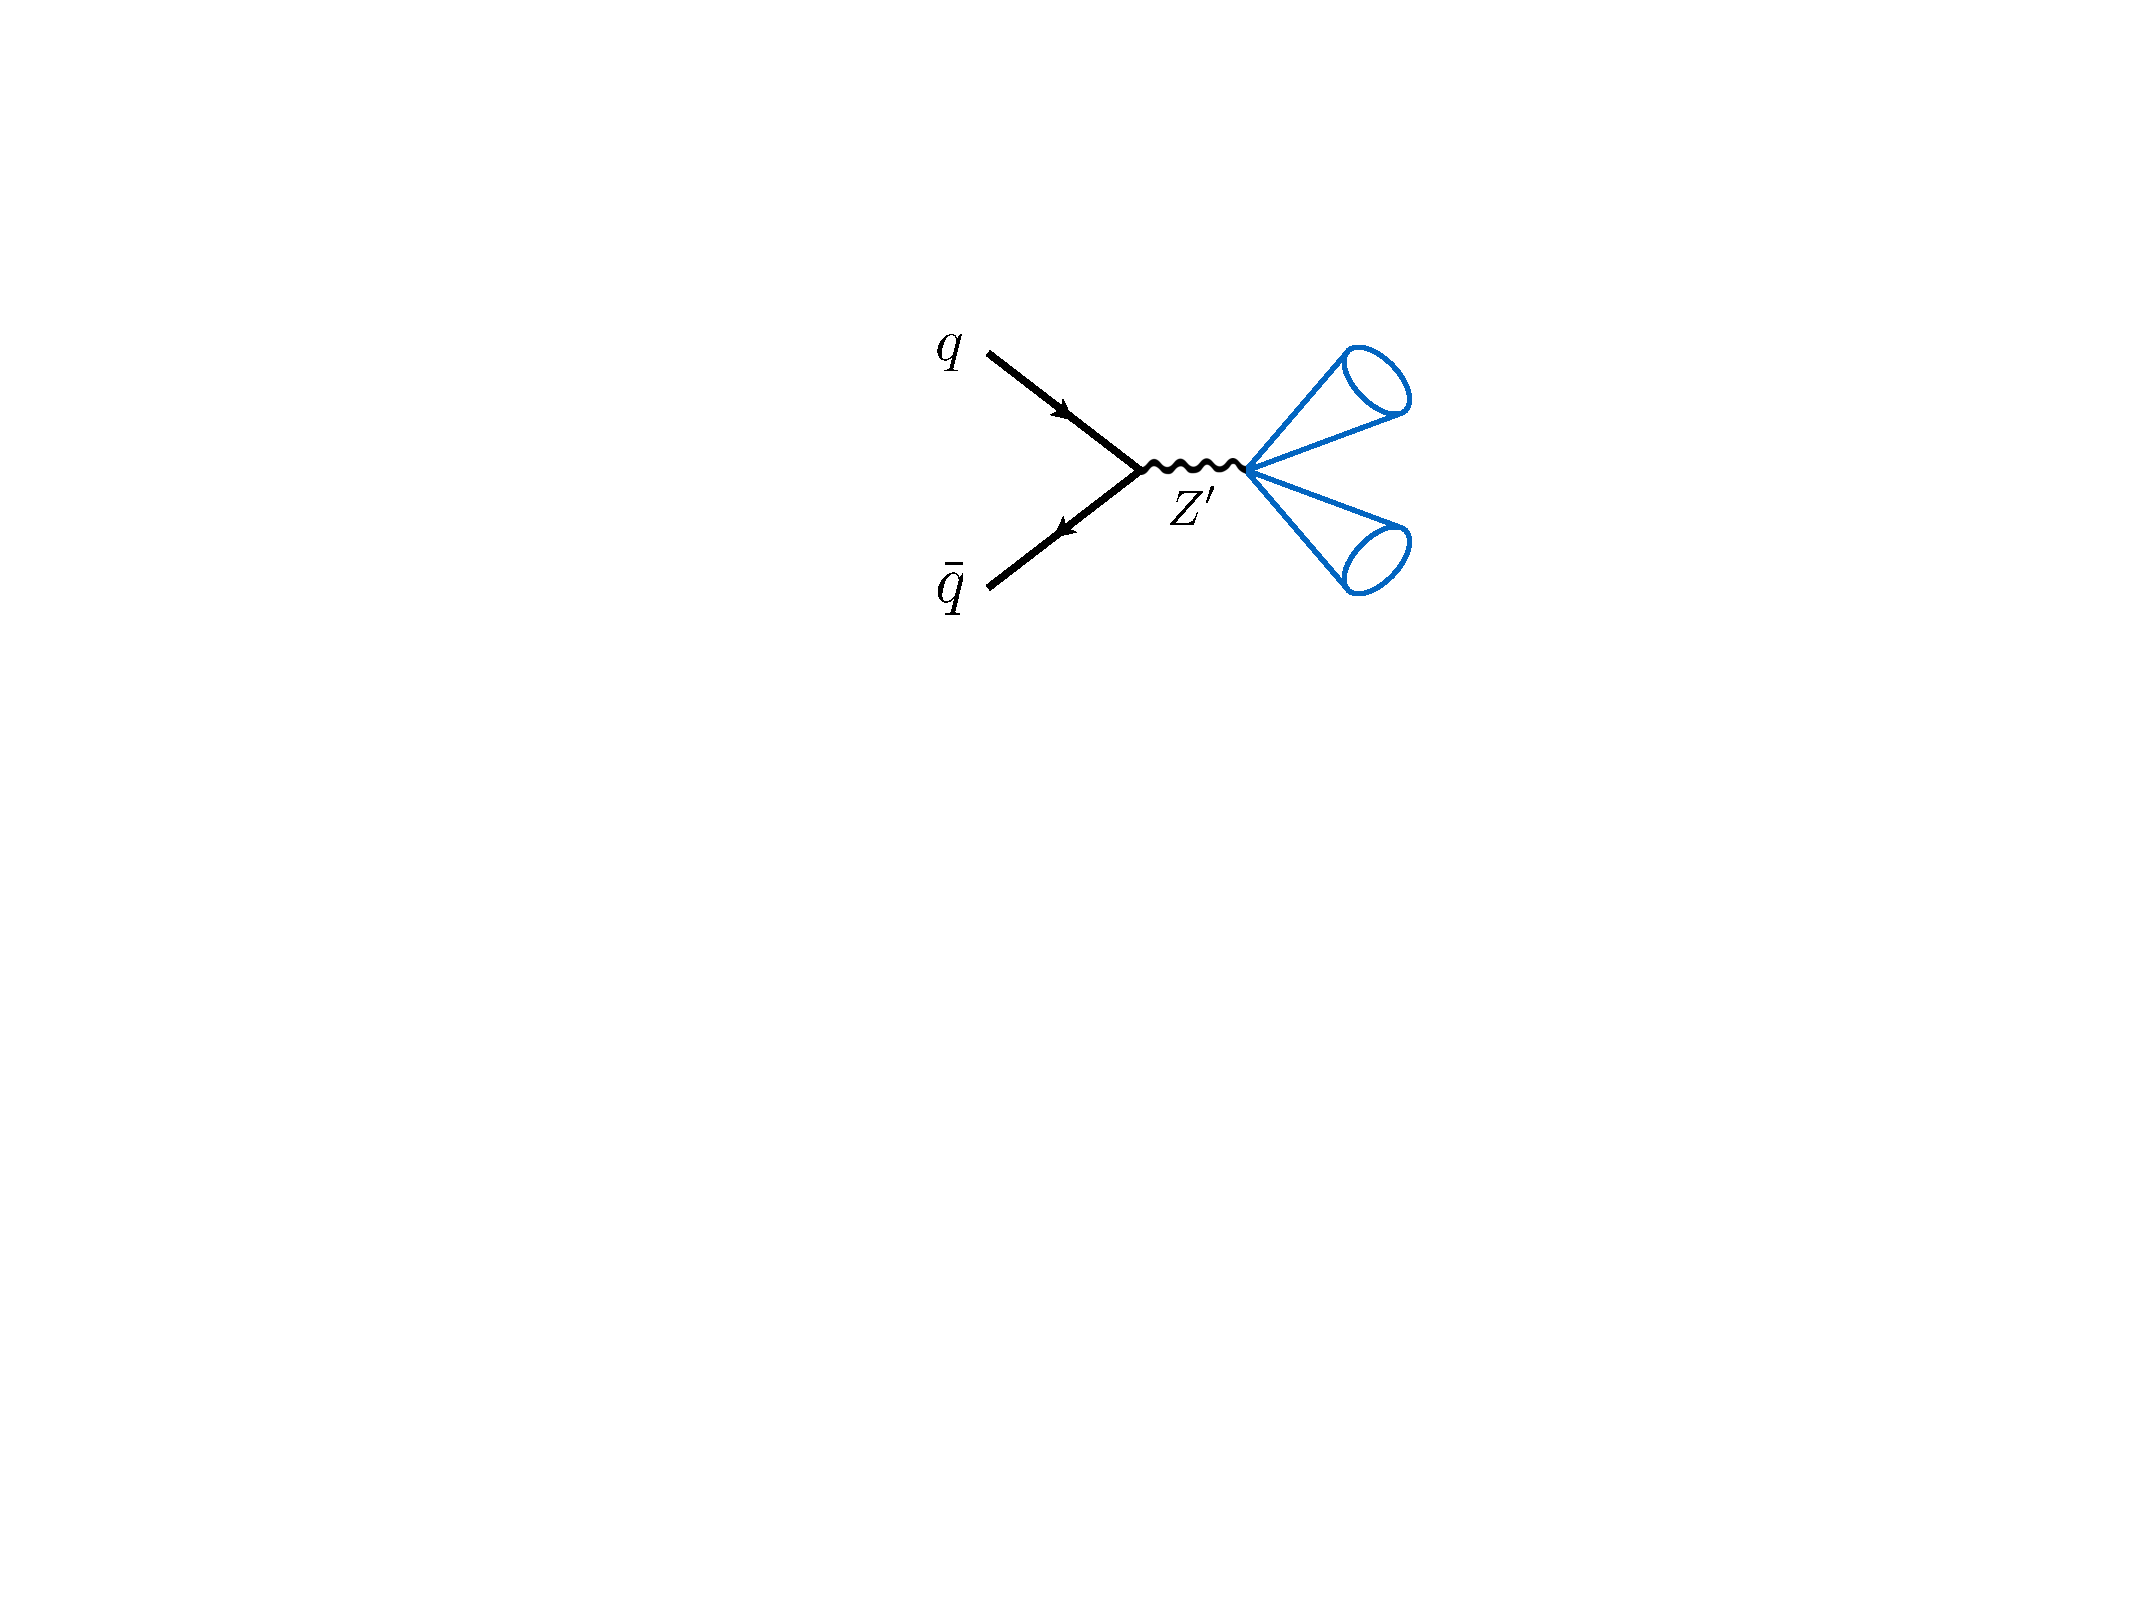
\includegraphics[width=0.7\textwidth]{figures/svj/portals_s.pdf}
        \caption{\schannel}
    \end{subfigure}
    \hfill
    \begin{subfigure}[c]{0.45\textwidth}
    \centering
        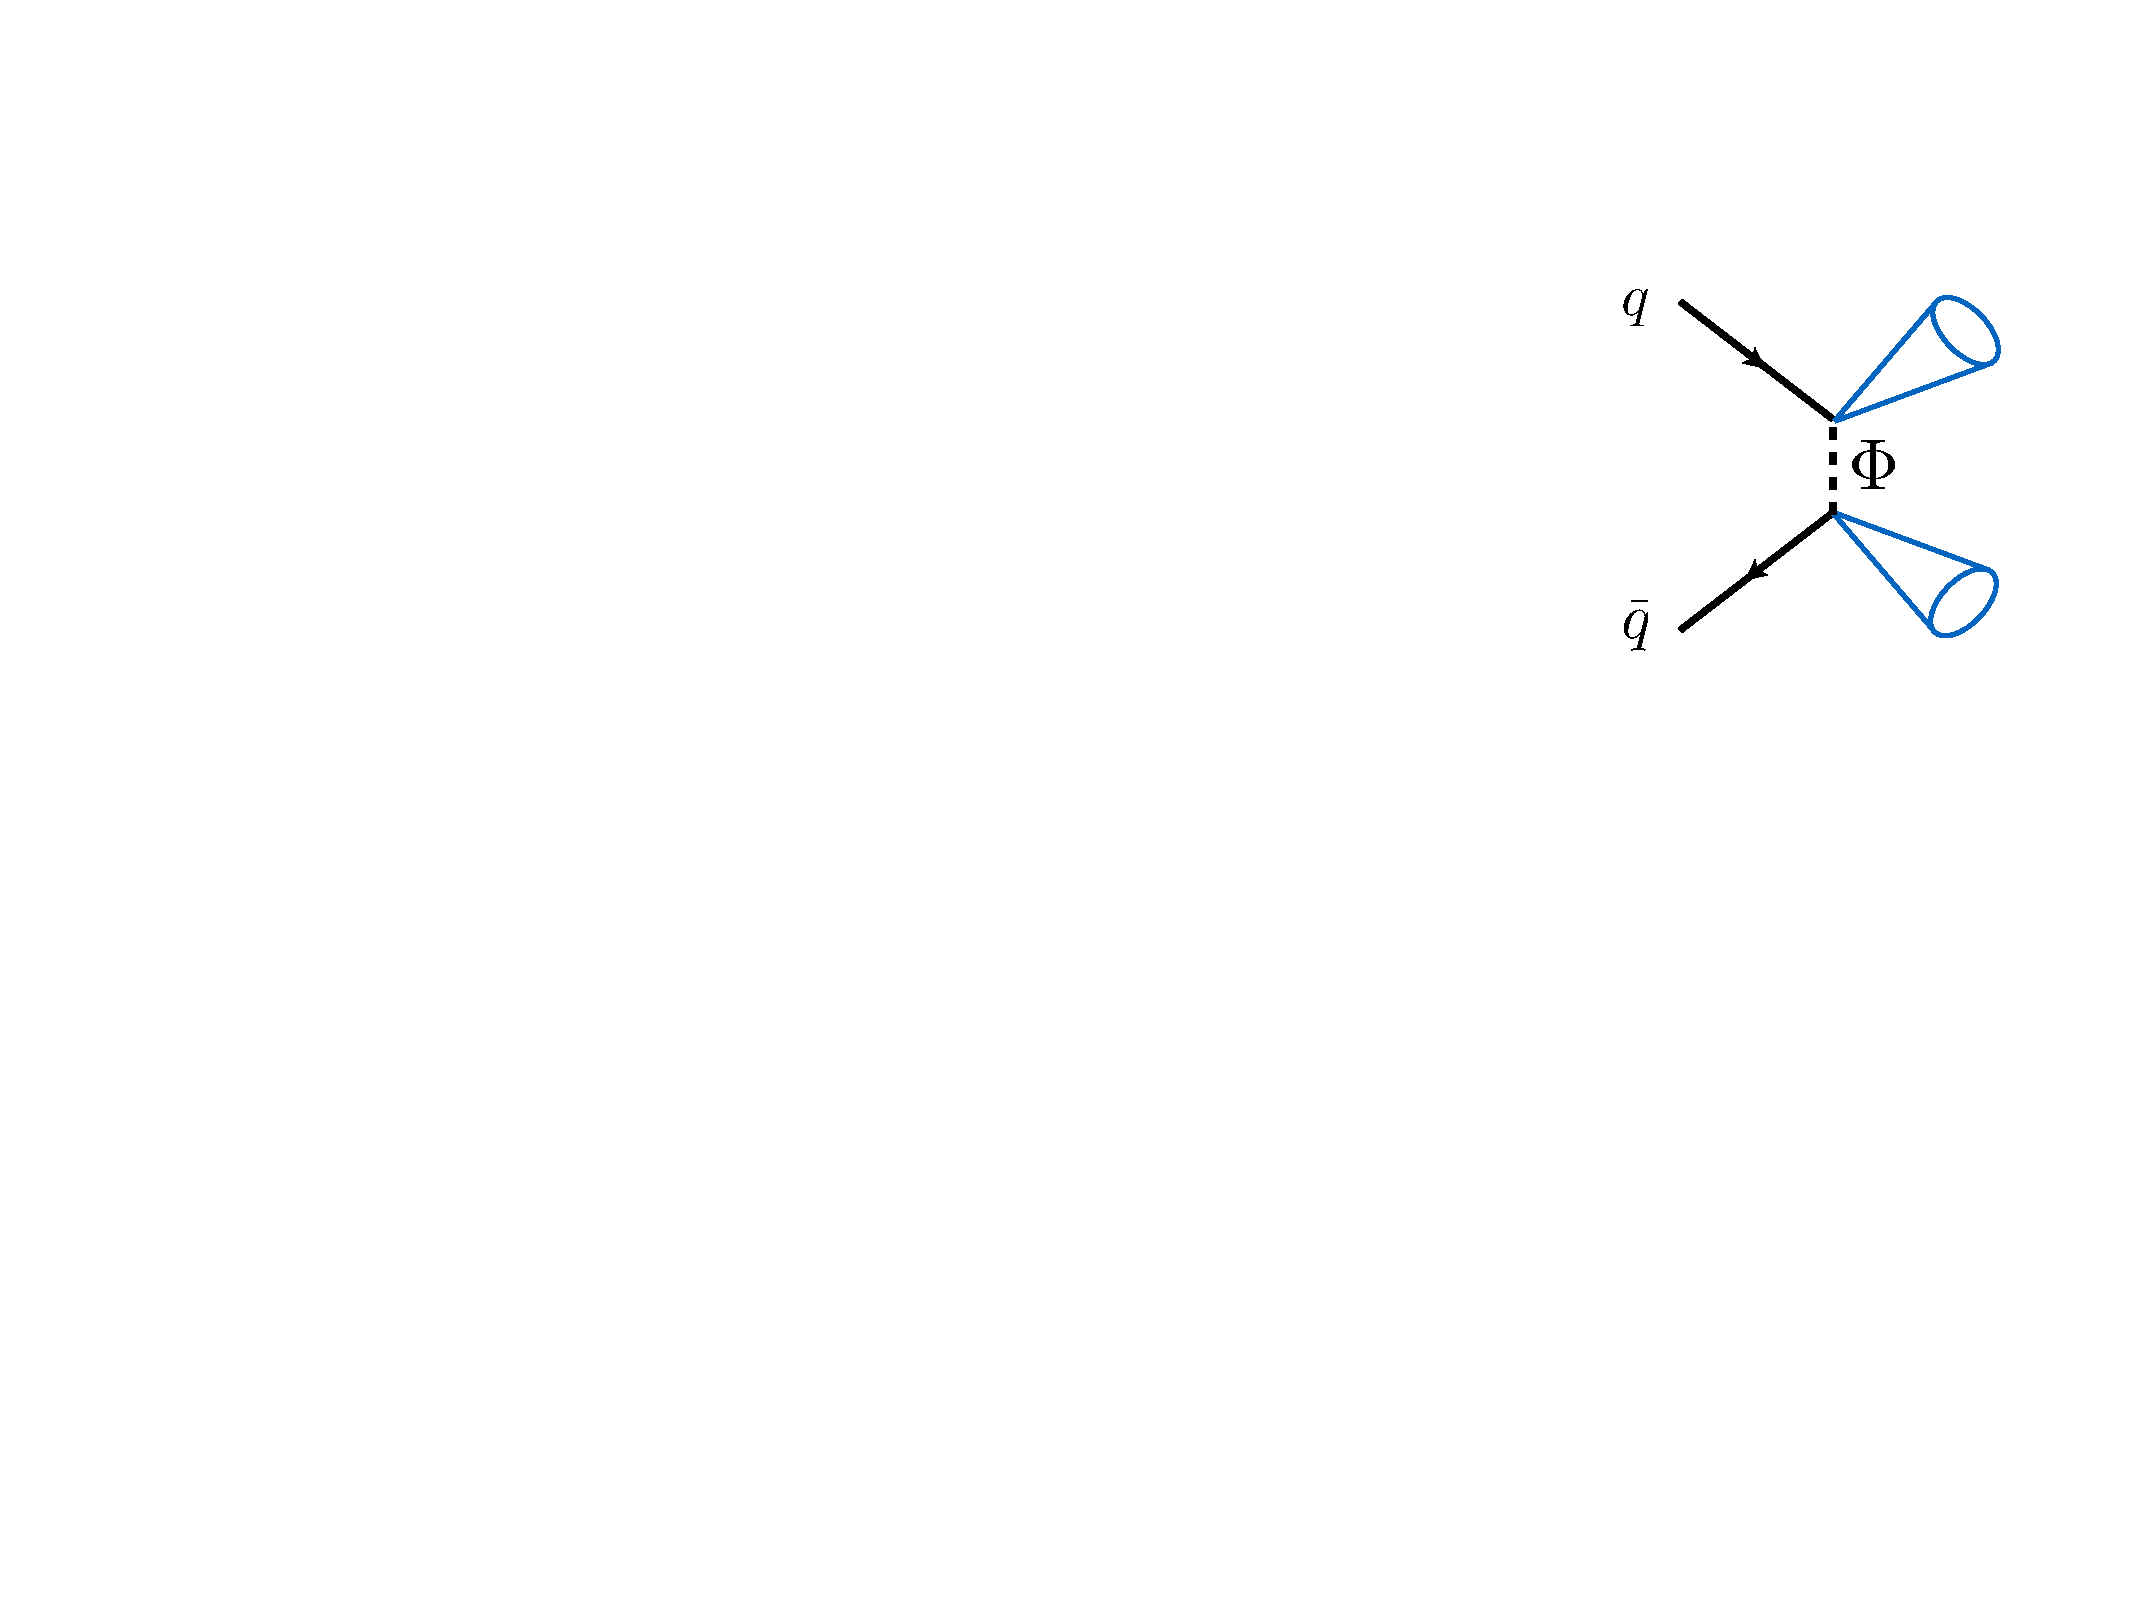
\includegraphics[width=0.7\textwidth]{figures/svj/portals_t.pdf}
        \caption{\tchannel}
    \end{subfigure}
\caption[Example Feynman diagrams for the two main production modes of semi-visible jets. A \PZprime  boson mediates the \schannel process while a bifundamental $\Phi$ mediates the \tchannel process]{Example Feynman diagrams for the two main production modes of semi-visible jets \cite{Cohen:2017pzm}. A \PZprime  boson mediates the \schannel process while a bifundamental $\Phi$ mediates the \tchannel process.}
\label{fig:theory_svj_portals}
\end{figure}

\begin{figure}[htbp]
\centering
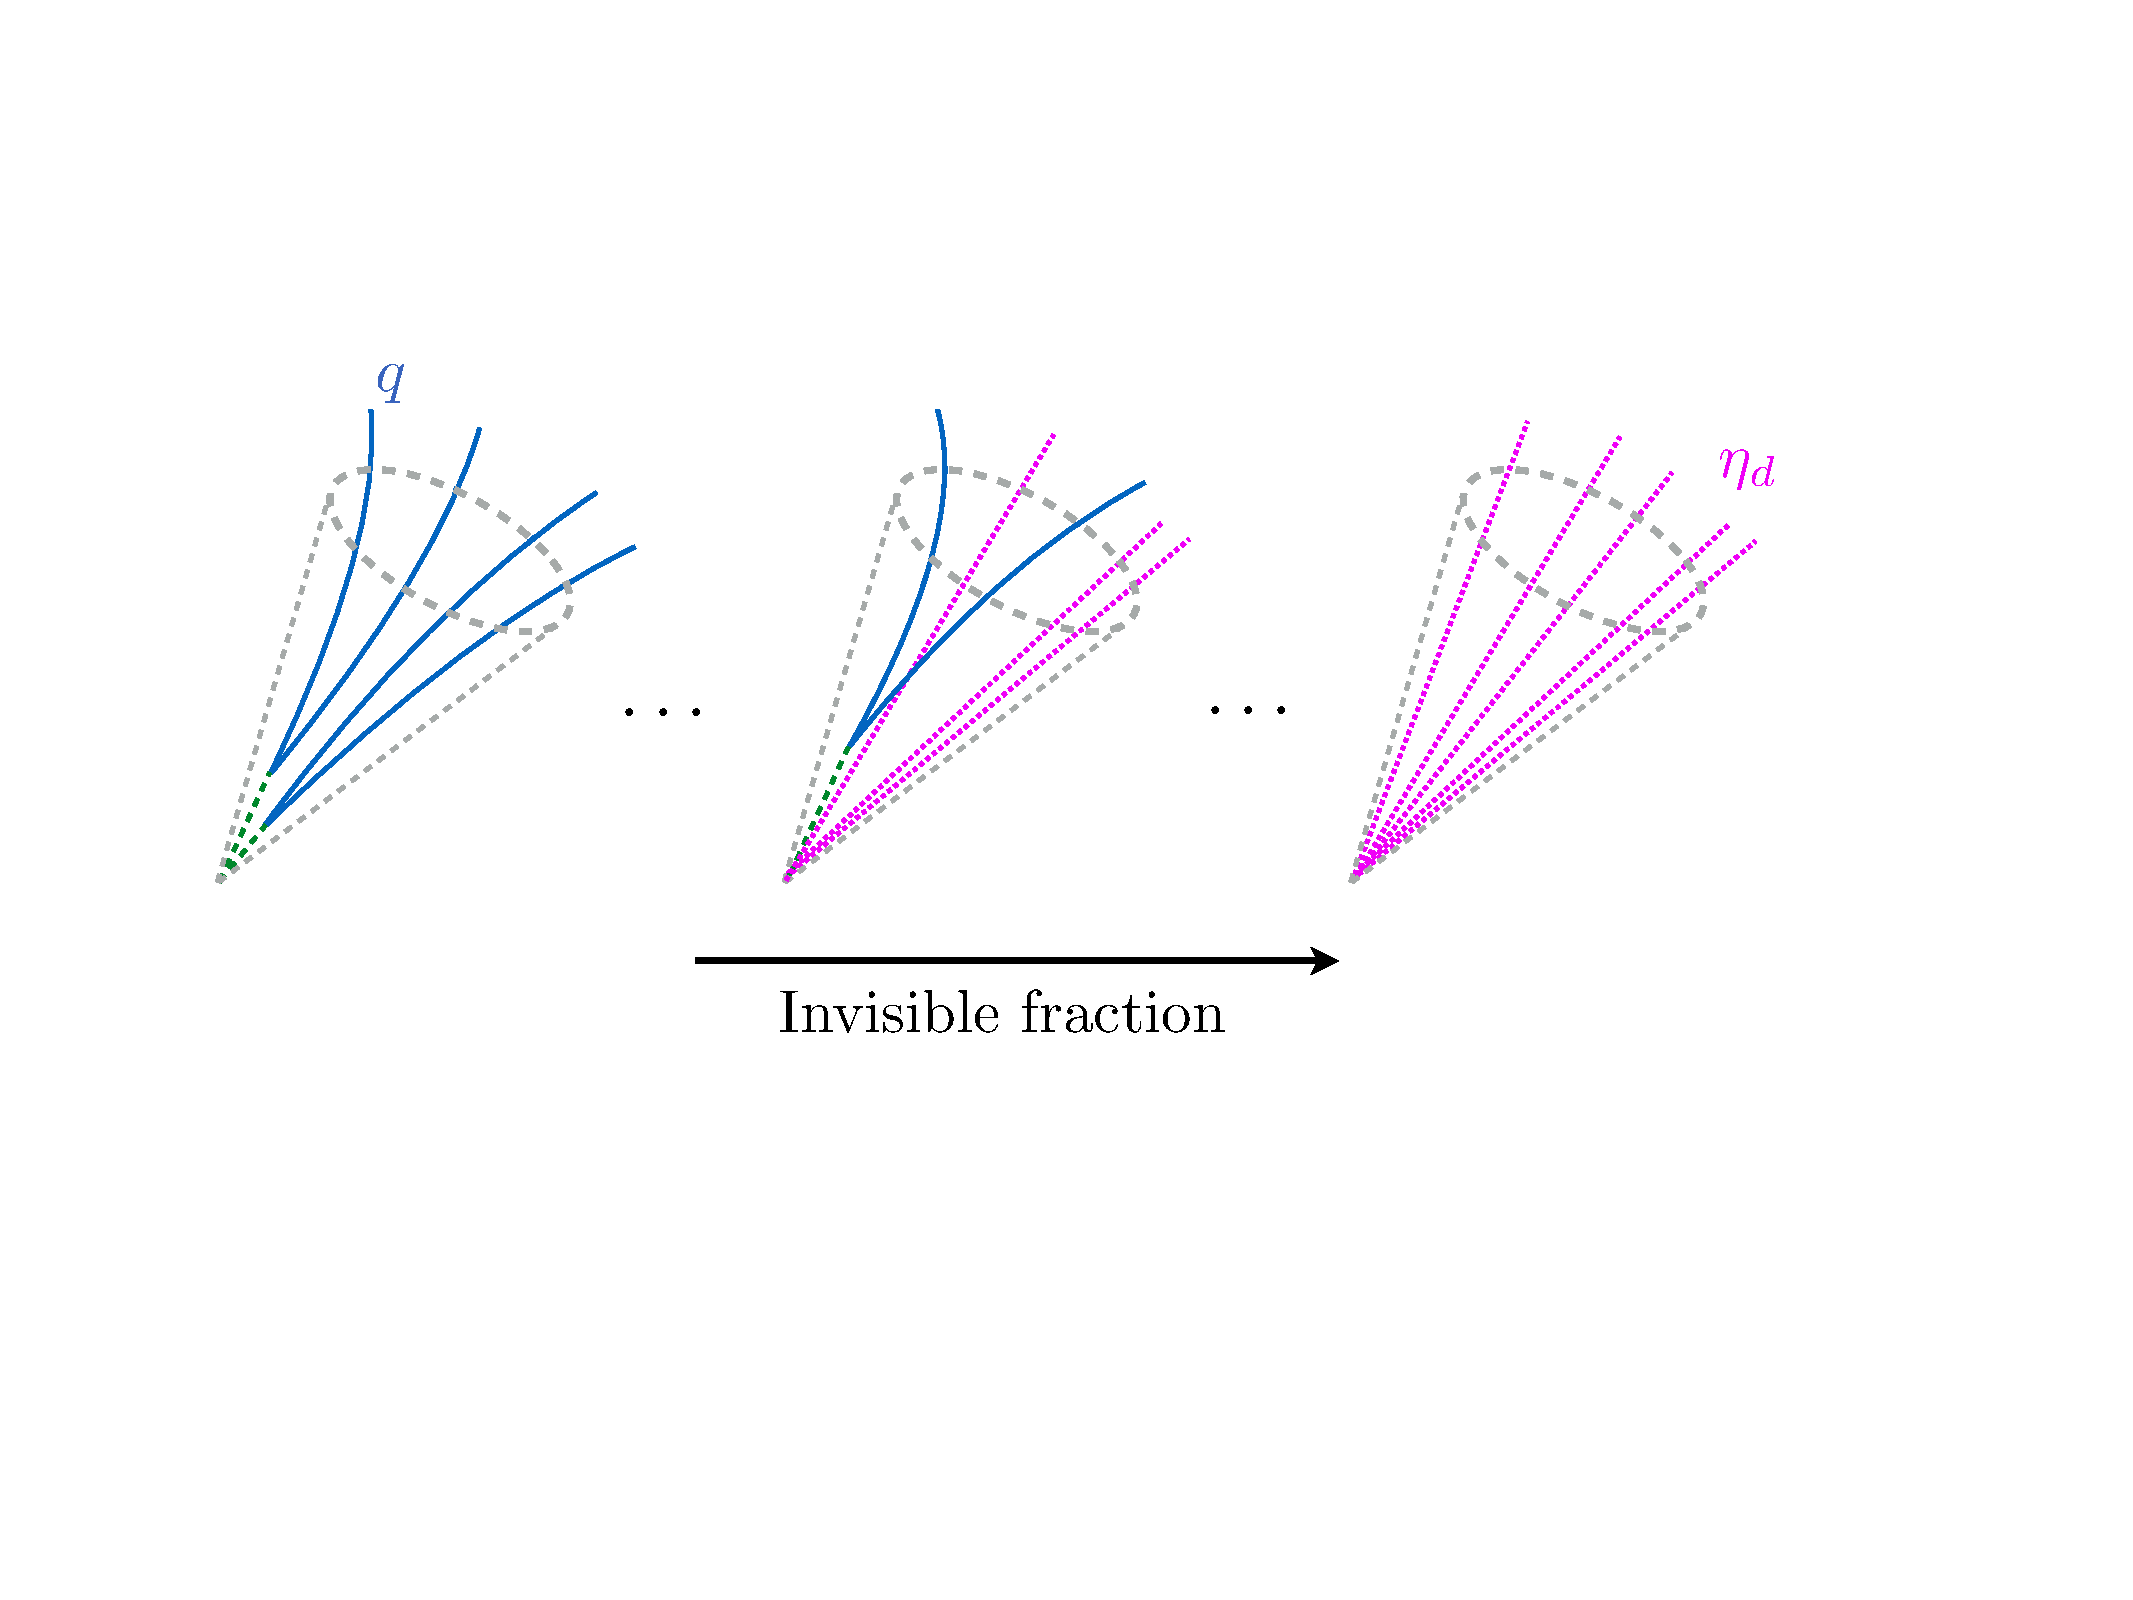
\includegraphics[width=0.75\textwidth]{figures/svj/r_inv.pdf}
\caption[The constituents of a semi-visible jet as a function of its invisible fraction]{The constituents of a semi-visible jet as a function of its invisible fraction \rinv \cite{Cohen:2017pzm}.}
\label{fig:theory_svj_rinv}
\end{figure}
